\documentclass[aspectratio=169,10pt]{beamer}

\usetheme{Madrid}
\usecolortheme{default}
\setbeamertemplate{navigation symbols}{}
\setbeamertemplate{footline}[frame number]

% 中文支持
\usepackage{ctex}
\setCJKmainfont{PingFang SC}
\setCJKsansfont{PingFang SC}

\usepackage{amsmath,amssymb,booktabs,mathtools}
\usepackage{graphicx}
\usepackage{hyperref}
\usepackage{tikz}
\usetikzlibrary{arrows.meta,positioning,decorations.pathreplacing}
\usepackage{pgfplots}
\pgfplotsset{compat=1.18}

% 语义颜色
\definecolor{positive}{HTML}{0173B2}
\definecolor{negative}{HTML}{DE8F05}
\definecolor{emphasis}{HTML}{029E73}
\definecolor{neutral}{gray}{0.55}
\definecolor{cbPurple}{HTML}{CC78BC}
\newcommand{\pos}[1]{\textcolor{positive}{#1}}
\newcommand{\con}[1]{\textcolor{negative}{#1}}
\newcommand{\HL}[1]{\textcolor{emphasis}{#1}}

% 自定义命令
\newcommand{\method}{PCD}
\newcommand{\taskspec}{TaskSpec}

\title{编译一次，精确推理\\[4pt]
{\normalsize LLM 概率推理的验证求解器诱导}}
\author{答辩人：姜博文 \quad 导师：姚涛}
\institute{上海交通大学 安泰经济与管理学院}
\date{2026}

\begin{document}

% ============================================================
% Slide 1: 封面
% ============================================================
\begin{frame}[plain]
\titlepage
\end{frame}

% ============================================================
% Slide 2: 动机
% ============================================================
\begin{frame}{动机：LLM 能理解概率问题，但算不对}
\vspace{4pt}

\textbf{一个令人困惑的现象}——以贝叶斯网络推理为例：

\vspace{6pt}
\begin{center}
\begin{tabular}{@{}p{7cm}cc@{}}
\toprule
\textbf{任务} & \textbf{GPT-5.4} & \textbf{困难？} \\
\midrule
提取网络结构（变量、边、CPT）& \pos{99\%} & 不难 \\
给定后验，选出最优决策 & \pos{100\%} & 不难 \\
\textbf{执行概率计算}（变量消去）& \con{11\%} {\scriptsize (depth=10)} & \textbf{很难} \\
\bottomrule
\end{tabular}
\end{center}

\vspace{4pt}
\begin{alertblock}{核心发现}
LLM \textbf{理解}问题结构、\textbf{会用}计算结果，但\textbf{算不对}中间的概率计算
\end{alertblock}

\vspace{4pt}
\begin{itemize}
    \item 跨 \textbf{6 个模型}（OpenAI / Anthropic / Google）、\textbf{5 个任务族}一致成立
    \item 升级到 GPT-5.4（67× 成本）仅提升 Compute 9pp，无法消除错误
\end{itemize}
\end{frame}

% ============================================================
% Slide 3: PCD 诊断方法
% ============================================================
\begin{frame}{PCD 诊断：三阶段分离}
\vspace{2pt}

\begin{center}
\begin{tikzpicture}[
    box/.style={draw, rounded corners=4pt, minimum width=2.4cm, minimum height=1cm,
                font=\small, thick, align=center}
]
    % 三个阶段
    \node[box, fill=positive!12] (P) at (0,0) {\textbf{Parse}\\[-2pt]{\scriptsize 提取问题结构}};
    \node[box, fill=negative!12] (C) at (5,0) {\textbf{Compute}\\[-2pt]{\scriptsize 概率计算}};
    \node[box, fill=emphasis!12] (D) at (10,0) {\textbf{Decide}\\[-2pt]{\scriptsize 做出决策}};

    % 箭头
    \draw[->, thick] (P) -- node[above, font=\scriptsize] {结构 $s^*$} (C);
    \draw[->, thick] (C) -- node[above, font=\scriptsize] {后验 $y^*$} (D);

    % 输入输出
    \node at (-2.2,0) [font=\small] {问题 $x$};
    \draw[->, thick] (-1.6,0) -- (P.west);
    \node at (12.2,0) [font=\small] {决策 $a^*$};
    \draw[->, thick] (D.east) -- (11.6,0);

    % Gold injection 标注
    \draw[dashed, thick, negative] (0,-1.0) -- (5,-1.0)
        node[midway, below=2pt, font=\scriptsize, text=negative] {注入金标准结构};
    \draw[dashed, thick, negative] (5,-1.0) -- (10,-1.0)
        node[midway, below=2pt, font=\scriptsize, text=negative] {注入金标准后验};

    % 准确率标注
    \node at (0,1.1) [font=\small, text=positive] {\textbf{82--100\%}};
    \node at (5,1.1) [font=\small, text=negative] {\textbf{22--78\%}};
    \node at (10,1.1) [font=\small, text=emphasis] {\textbf{100\%}};
\end{tikzpicture}
\end{center}

\vspace{4pt}

\textbf{方法}：通过注入金标准中间结果，\textbf{隔离每个阶段的误差}

\begin{itemize}
    \item \textbf{Parse}：LLM 能否正确提取问题结构？→ 逐字段对比
    \item \textbf{Compute$\mid$GoldParse}：给定完美结构，LLM 能否正确计算？→ 数值对比 ($\epsilon < 0.01$)
    \item \textbf{Decide$\mid$GoldPosterior}：给定完美后验，LLM 能否正确决策？→ 精确匹配
\end{itemize}
\end{frame}

% ============================================================
% Slide 4: PCD 结果
% ============================================================
\begin{frame}{PCD 结果：计算是普遍瓶颈}
\vspace{2pt}

\begin{columns}[T]
\column{0.38\textwidth}
{\small \textbf{偏好学习 PCD}（Flight, $n{=}200$）}

\vspace{4pt}
{\small
\begin{tabular}{@{}lcc@{}}
\toprule
模型 & Parse & Compute \\
\midrule
GPT-4o-mini & 82\% & \con{28\%} \\
GPT-4o & 100\% & \con{30\%} \\
GPT-5.4 & 100\% & \con{40\%} \\
Sonnet 4 & 100\% & 64\% \\
Gemini 3.1 & 100\% & 69\% \\
Opus 4.6 & 100\% & 78\% \\
\midrule
Our DSL & --- & \pos{100\%} \\
\bottomrule
\end{tabular}}

\vspace{4pt}
{\scriptsize 所有模型 Decide = 100\%}

\column{0.60\textwidth}
{\small \textbf{BN 推理 Compute 随深度急剧下降}}

\vspace{2pt}
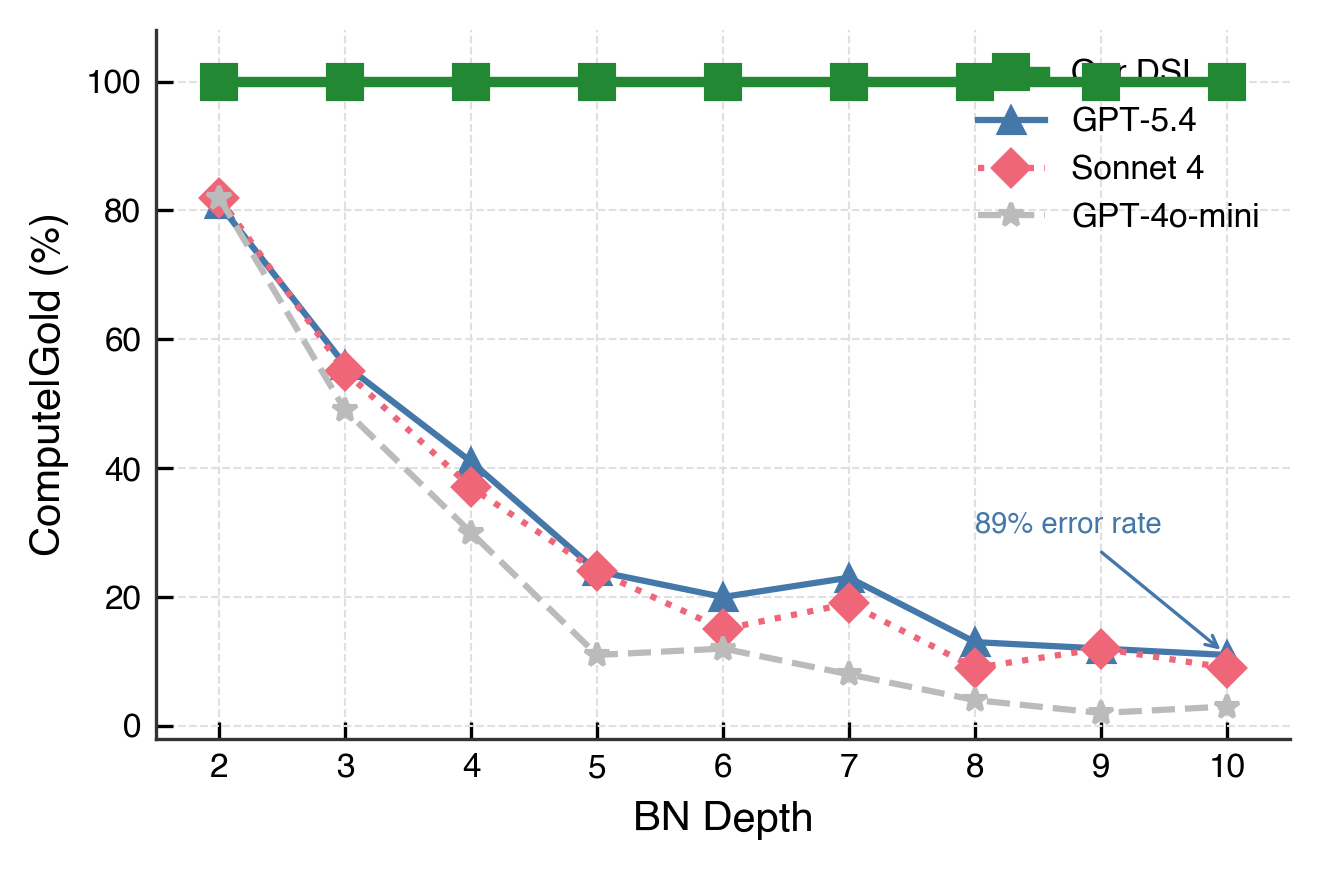
\includegraphics[width=\textwidth]{figures/figure2_depth.png}

{\scriptsize GPT-5.4 depth=10 仅 11\%，升级模型 67× 成本仅提升 9pp}
\end{columns}
\end{frame}

% ============================================================
% Slide 5: 系统架构
% ============================================================
\begin{frame}{方法：Compile-Once 求解器诱导}
\vspace{2pt}

\begin{center}
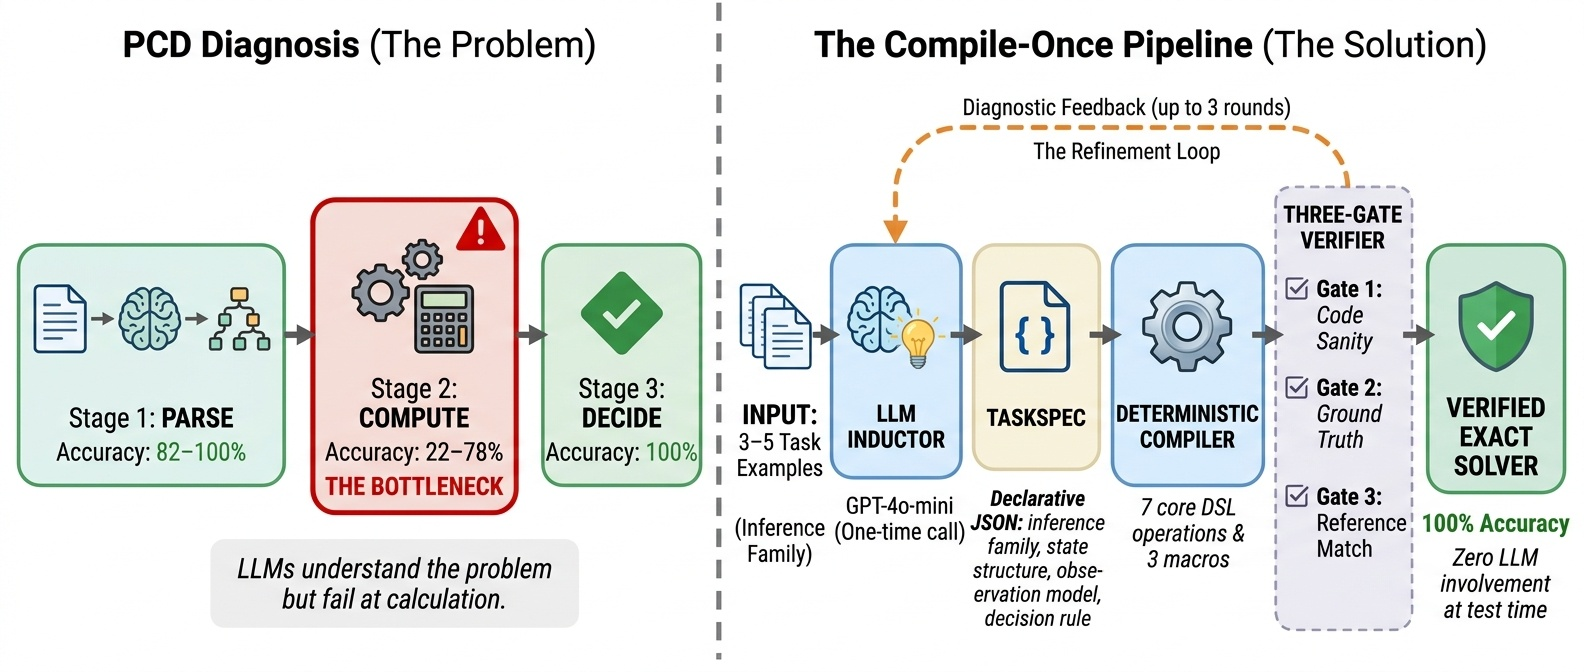
\includegraphics[width=0.95\textwidth]{figures/figure1_overview.png}
\end{center}

\vspace{2pt}

{\small
\textbf{左}：PCD 诊断发现计算是瓶颈 \quad
\textbf{右}：LLM 诱导 TaskSpec → 编译器生成精确求解器 → 三门验证器把关
\par
\textbf{关键}：LLM 只调用\textbf{一次}（per family），之后所有推理\textbf{零 LLM 成本}、\textbf{确定性}输出
}
\end{frame}

% ============================================================
% Slide 6: DSL 设计
% ============================================================
\begin{frame}{概率 DSL：7 个核心运算 + 3 个宏}
\vspace{2pt}

\begin{columns}[T]
\column{0.48\textwidth}
\begin{exampleblock}{核心运算（typed ops）}
{\small
\texttt{condition} · \texttt{multiply} · \texttt{marginalize}\\
\texttt{normalize} · \texttt{enumerate\_hypotheses}\\
\texttt{expectation} · \texttt{argmax}\\[4pt]
每个运算有精确类型签名\\
例：\texttt{normalize: Factor $\to$ Distribution}
}
\end{exampleblock}

\vspace{4pt}
\textbf{为什么 LLM 只需填 JSON？}
\begin{itemize}
    \item 声明结构，不写代码 → 消除语法错误
    \item \pos{GPT-4o-mini 即可胜任}（40/40 次一次通过）
\end{itemize}

\column{0.48\textwidth}
\begin{exampleblock}{Family Macros（语法糖）}
{\small
\texttt{softmax\_pref}：假设枚举\\
\texttt{beta\_bernoulli}：共轭更新\\
\texttt{ve\_query}：变量消去\\[4pt]
宏 = 核心运算的组合\\
\textbf{非必需}：无宏也达 100\%
}
\end{exampleblock}

\vspace{4pt}
\textbf{编译器保证}：
\begin{itemize}
    \item 确定性：同一 spec $\to$ 同一 solver
    \item 等价性：1,200 样本 max error = \pos{0.0}
\end{itemize}
\end{columns}
\end{frame}

% ============================================================
% Slide 7: BN 实验结果
% ============================================================
\begin{frame}{实验：合成网络 + 真实世界网络}
\vspace{2pt}

\begin{columns}[T]
\column{0.52\textwidth}
{\small \textbf{bnlearn 真实网络}（8--37 节点）}

\vspace{2pt}
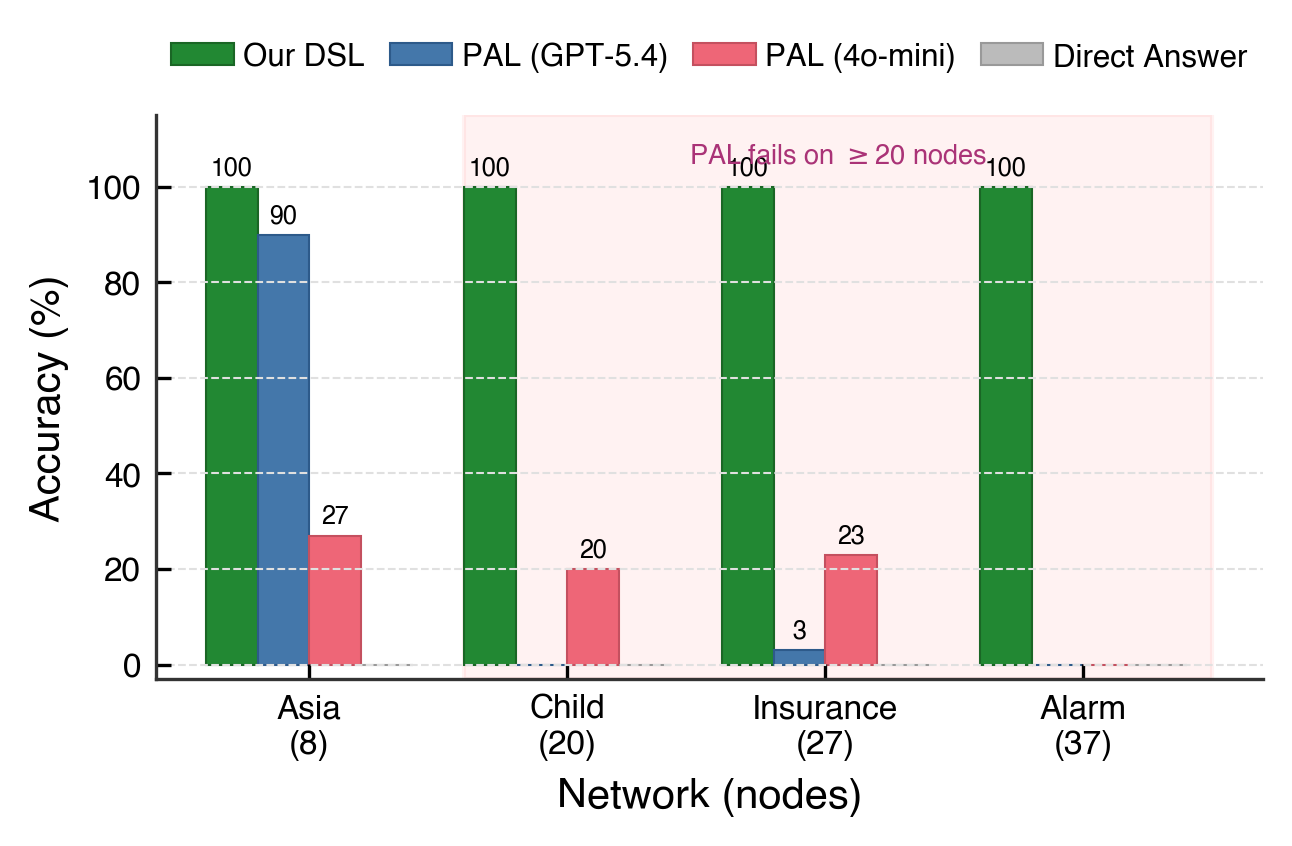
\includegraphics[width=\textwidth]{figures/figure3a_bnlearn.png}

{\scriptsize $\geq$20 节点：PAL $\to$ 0--3\%，DSL 保持 \pos{100\%}}

\column{0.46\textwidth}
{\small \textbf{关键发现}}

\vspace{6pt}
\begin{itemize}
    \item BLInD 合成网络：PAL (mini) 从 93\% 降至 2\%
    \item \textbf{PAL 的核心问题}：生成的 VE 代码在多值 CPT、深消去链上崩溃
    \item 我们的 DSL：\textbf{同一个} \texttt{ve\_query} 宏覆盖所有网络
    \item 无需额外诱导：BLInD 编译的 solver 直接应用于 bnlearn
\end{itemize}

\vspace{4pt}
\begin{alertblock}{\small 规模越大，优势越大}
{\small 小网络差 2pp → 大网络差 $\sim$100pp}
\end{alertblock}
\end{columns}
\end{frame}

% ============================================================
% Slide 8: 成本与泛化
% ============================================================
\begin{frame}{成本优势 \& 泛化到未见任务族}
\vspace{2pt}

\begin{columns}[T]
\column{0.48\textwidth}
{\small \textbf{成本--准确率 Pareto 前沿}}

\vspace{2pt}
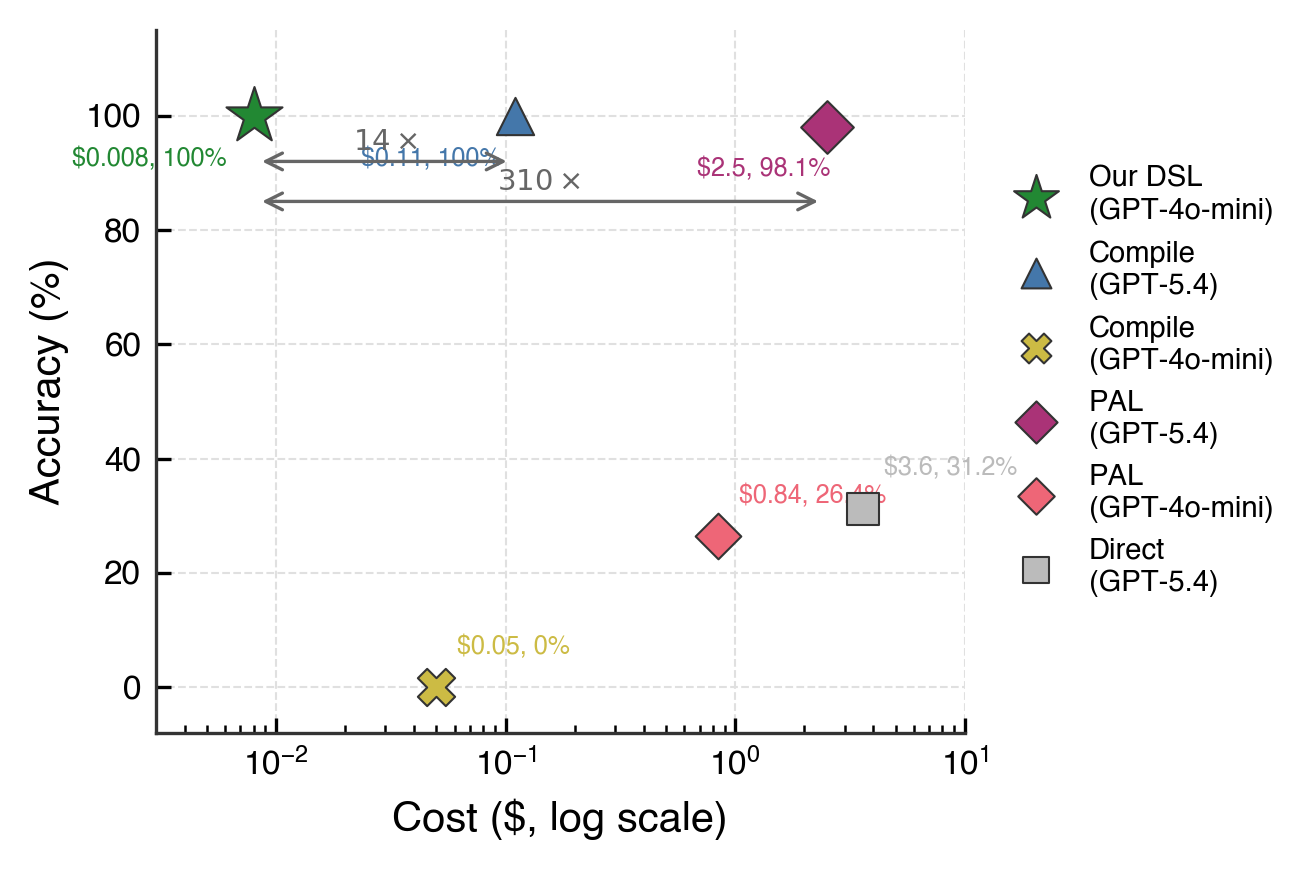
\includegraphics[width=\textwidth]{figures/figure3b_cost.png}

{\scriptsize GPT-4o-mini \$0.008 = GPT-5.4 Compile 的 1/14 成本}

\column{0.48\textwidth}
{\small \textbf{Held-out 家族}（无对应宏）}

\vspace{4pt}
{\small
\begin{tabular}{@{}lcc@{}}
\toprule
 & NB & HMM \\
\midrule
Direct (mini) & 44\% & 32\% \\
Direct (5.4) & 69\% & 61\% \\
\midrule
Free Code & \pos{100\%} & \pos{100\%} \\
\textbf{Core-ops} & \pos{100\%} & \pos{100\%} \\
\bottomrule
\end{tabular}}

\vspace{6pt}
\begin{itemize}
    \item \textbf{HMM}：需要时序迭代 multiply--marginalize--normalize，训练宏中不存在此模式
    \item 核心运算\textbf{自动组合}出新的推理流程
\end{itemize}
\end{columns}
\end{frame}

% ============================================================
% Slide 9: 端到端 & 策略消融
% ============================================================
\begin{frame}{端到端验证 \& 23 策略消融}
\vspace{2pt}

\begin{columns}[T]
\column{0.48\textwidth}
\begin{alertblock}{\small 端到端 Pipeline（偏好学习）}
{\small
自然语言航班描述 → LLM Parse → 编译求解器 → 推荐

\vspace{4pt}
\textbf{准确率}：\pos{74.3\%} [70.9, 77.8]\\
Gold Oracle：74.4\%\\[2pt]
特征提取准确率：99.9--100\%\\
与 Gold Solver 一致率：99.8\%
}
\end{alertblock}

\vspace{4pt}
{\small 对比最佳 prompt 策略（tool-calling 58.3\%）\\
→ \textbf{+16pp} 提升}

\column{0.48\textwidth}
{\small \textbf{23 策略消融：计算 offload 越多越好}}

\vspace{4pt}
\begin{tikzpicture}[xscale=0.85, yscale=0.045]
    % 坐标轴
    \draw[-{Stealth}, thick] (0,0) -- (0,82) node[above, font=\scriptsize] {准确率};
    \draw[-{Stealth}, thick] (0,0) -- (6.5,0) node[right, font=\scriptsize] {offload 程度};

    % 数据条
    \fill[neutral!40] (0.5,0) rectangle (1.2,33);
    \node[above, font=\tiny] at (0.85,33) {33\%};
    \node[below, font=\tiny, text width=1cm, align=center] at (0.85,0) {纯\\CoT};

    \fill[negative!50] (1.8,0) rectangle (2.5,50);
    \node[above, font=\tiny] at (2.15,50) {50\%};
    \node[below, font=\tiny, text width=1cm, align=center] at (2.15,0) {数学\\注入};

    \fill[positive!50] (3.1,0) rectangle (3.8,58);
    \node[above, font=\tiny] at (3.45,58) {58\%};
    \node[below, font=\tiny, text width=1.2cm, align=center] at (3.45,0) {工具\\调用};

    \fill[emphasis!60] (4.4,0) rectangle (5.1,74.3);
    \node[above, font=\tiny] at (4.75,74.3) {\textbf{74.3\%}};
    \node[below, font=\tiny, text width=1.2cm, align=center] at (4.75,0) {编译\\求解器};

    \draw[dashed, neutral] (0, 74.8) -- (5.8, 74.8)
        node[right, font=\tiny, text=neutral] {Oracle};
\end{tikzpicture}

\vspace{2pt}
{\scriptsize 梯度单调：LLM 做的数学越少，准确率越高}
\end{columns}
\end{frame}

% ============================================================
% Slide 10: 总结
% ============================================================
\begin{frame}{总结与展望}
\vspace{4pt}

\textbf{核心贡献}

\begin{enumerate}
    \item \textbf{PCD 诊断}：6 模型 × 5 任务族证明\textbf{计算是唯一瓶颈}\\
    {\small Parse $\geq$82\%, Decide = 100\%, Compute 仅 22--78\%}

    \item \textbf{Compile-Once 系统}：7 运算 DSL + 编译器 + 三门验证器\\
    {\small GPT-4o-mini 生成 100\% 准确求解器，成本 \$0.008（GPT-5.4 PAL 的 1/310）}
\end{enumerate}

\vspace{6pt}
\textbf{更广泛的原则}

\begin{center}
\begin{tikzpicture}[
    box/.style={draw, rounded corners=3pt, minimum height=0.7cm, font=\small, thick}
]
    \node[box, fill=positive!12, minimum width=3.2cm] (llm) {LLM：语言理解};
    \node[box, fill=emphasis!12, minimum width=3.8cm, right=1.2cm of llm] (solver) {确定性后端：精确计算};
    \draw[-{Stealth}, thick] (llm) -- node[above, font=\scriptsize] {结构} (solver);
\end{tikzpicture}
\end{center}

\vspace{4pt}
\textbf{局限}：仅覆盖离散精确推理，不处理连续变量或预测型任务

\textbf{未来}：连续分布扩展、近似推理后端、更多任务族验证
\end{frame}

% ============================================================
% Slide 11: 参考文献
% ============================================================
\begin{frame}{参考文献}
\small
\begin{thebibliography}{9}
\bibitem{nafar2025blind} Nafar et al. (2025). BLInD: Blind LLM Inference Diagnostics for Bayesian Networks. \textit{AAAI}.
\bibitem{gao2023pal} Gao et al. (2023). PAL: Program-Aided Language Models. \textit{ICML}.
\bibitem{qiu2026bayesian} Qiu et al. (2026). Bayesian Teaching Enables Probabilistic Reasoning in LLMs. \textit{Nature Communications}.
\bibitem{schrader2024quite} Schrader \& Thieme (2024). QUITE: Quantifying Uncertainty in Natural Language Text. \textit{NeurIPS}.
\bibitem{ellis2021dreamcoder} Ellis et al. (2021). DreamCoder: Bootstrapping Inductive Program Synthesis. \textit{PLDI}.
\bibitem{koller2009pgm} Koller \& Friedman (2009). \textit{Probabilistic Graphical Models}. MIT Press.
\end{thebibliography}
\end{frame}

% ============================================================
% Slide 12: 致谢
% ============================================================
\begin{frame}[plain]
\vfill
\begin{center}
{\Huge 谢谢！}

\vspace{12pt}
{\large 欢迎提问与讨论}

\vspace{20pt}
{\small 姜博文 \quad tree06@sjtu.edu.cn\\[4pt]
上海交通大学 安泰经济与管理学院}
\end{center}
\vfill
\end{frame}

% ============================================================
% Backup Slides
% ============================================================
\appendix

\begin{frame}{Backup Slides}
\end{frame}

% ============================================================
% Backup 1: PCD 形式化
% ============================================================
\begin{frame}{Backup: PCD 形式化定义}
\vspace{2pt}

对于问题实例 $x$，金标准计算流水线：
\[
s^* = \mathcal{P}^*(x), \quad y^* = \mathcal{C}^*(s^*), \quad a^* = \mathcal{D}^*(y^*)
\]

PCD 通过注入金标准中间结果隔离每个阶段：
\begin{align}
\text{ParseAcc}_\phi &= \frac{1}{|\mathcal{D}|}\sum_{x \in \mathcal{D}} \prod_{f \in \mathcal{F}} \mathbf{1}\!\left\{P_\phi^{(f)}(x) = s^{*(f)}\right\} \\[4pt]
\text{CompAcc}_\phi &= \frac{1}{|\mathcal{D}|}\sum_{x \in \mathcal{D}} \mathbf{1}\!\left\{\left\|C_\phi\!\left(\mathcal{P}^*(x)\right) - \mathcal{C}^*\!\left(\mathcal{P}^*(x)\right)\right\|_\infty < \epsilon\right\} \\[4pt]
\text{DecAcc}_\phi &= \frac{1}{|\mathcal{D}|}\sum_{x \in \mathcal{D}} \mathbf{1}\!\left\{D_\phi\!\left(\mathcal{C}^*(s^*)\right) = a^*\right\}
\end{align}

当 $\text{ParseAcc} \approx 1,\; \text{DecAcc} \approx 1,\; \text{CompAcc} \ll 1$ 时，确认\textbf{计算瓶颈}
\end{frame}

% ============================================================
% Backup 2: 23 策略完整表
% ============================================================
\begin{frame}{Backup: 23 策略消融完整结果}
\vspace{2pt}

{\scriptsize
\begin{center}
\begin{tabular}{@{}llcc@{}}
\toprule
类别 & 策略 & 准确率 & 服从率 \\
\midrule
对照组 & baseline & 36.8\% & --- \\
 & random\_rec & 33.5\% & 33.7\% \\
\midrule
纯 CoT & 4 种变体 & 32--33\% & 32--33\% \\
\midrule
Prompt 注入 & direct\_rec & 34.8\% & 39.5\% \\
 & nl\_pref\_rec & 38.8\% & 51.4\% \\
 & full\_math & 49.9\% & 67.7\% \\
\midrule
混合策略 & cot\_then\_math & 49.5\% & 68.7\% \\
 & math\_then\_cot & 40.9\% & 49.0\% \\
\midrule
工具调用 & tool\_empty & 37.1\% & 37.1\% \\
 & tool\_random\_rec & 36.3\% & 36.0\% \\
 & tool\_direct\_rec & 53.5\% & 81.6\% \\
 & tool\_nl\_pref\_rec & 56.8\% & 85.9\% \\
 & tool\_use (full) & \textbf{58.3\%} & 89.9\% \\
\midrule
编译求解器 & compile-once & \textbf{74.3\%} & --- \\
Oracle & gold posterior & 74.8\% & --- \\
\bottomrule
\end{tabular}
\end{center}}

{\scriptsize GPT-4o-mini, Flight 624 样本。服从率与准确率相关系数 $r = 0.97$}
\end{frame}

% ============================================================
% Backup 3: DSL 等价性 & LOO
% ============================================================
\begin{frame}{Backup: DSL 等价性验证 \& LOO 泛化}
\vspace{2pt}

\begin{columns}[T]
\column{0.48\textwidth}
\begin{exampleblock}{等价性验证}
{\small
\begin{tabular}{@{}lcc@{}}
\toprule
数据集 & 样本数 & Max Error \\
\midrule
Flight & 250 & \pos{0.0} \\
BLInD & 900 & \pos{0.0} \\
TextBandit & 50 & \pos{0.0} \\
\bottomrule
\end{tabular}

\vspace{4pt}
交叉验证：与 pgmpy 独立实现对比
}
\end{exampleblock}

\column{0.48\textwidth}
\begin{exampleblock}{LOO 泛化测试}
{\small
\begin{tabular}{@{}lc@{}}
\toprule
Held-out 数据集 & 通过轮次 \\
\midrule
Hotel & 第 1 轮 \\
Flight-2F/3F/5F/6F & 第 1 轮 \\
BLInD depth-OOD & 第 1 轮 \\
\bottomrule
\end{tabular}

\vspace{4pt}
6/6 首次通过，无需 self-refine\\
Gate 3 Off ablation：仍 100\%
}
\end{exampleblock}
\end{columns}

\vspace{6pt}
\textbf{Inductor 可靠性}：20 次/family × 2 families = 40 次，temperature 0.7，全部首次通过
\end{frame}

% ============================================================
% Backup 4: Applicability Boundary
% ============================================================
\begin{frame}{Backup: 适用边界 — DeLLMa 案例}
\vspace{4pt}

\textbf{并非所有概率任务都是计算瓶颈型}

\vspace{6pt}
\begin{itemize}
    \item \textbf{DeLLMa}：LLM 选择农业策略应对天气不确定性
    \item 编译求解器准确率：17--29\%（$\approx$ 随机基线 29\%）
    \item \con{原因}：DeLLMa 的瓶颈是\textbf{从历史数据估计分布}，不是计算已知分布
\end{itemize}

\vspace{8pt}

\begin{center}
\begin{tikzpicture}[
    box/.style={draw, rounded corners=3pt, minimum height=0.8cm, font=\small, thick, text width=4.5cm, align=center}
]
    \node[box, fill=emphasis!15] (works) {\pos{有效}：分布已给定或可推导\\BN / 偏好学习 / Bandit / NB / HMM};
    \node[box, fill=negative!15, right=1.5cm of works] (fails) {\con{无效}：瓶颈是预测而非计算\\DeLLMa (农业决策)};
\end{tikzpicture}
\end{center}

\vspace{6pt}
{\small 我们的 DSL 在\textbf{计算瓶颈}存在时有效，在\textbf{预测瓶颈}时无效}
\end{frame}

\end{document}
